\documentclass[12pt,a4paper,]{book}
\def\ifdoblecara{} %% set to true
\def\ifprincipal{} %% set to true
\def\ifcitapandoc{} %% set to true
\let\ifcitapandoc\undefined %% set to false
\usepackage{lmodern}
\usepackage{amssymb,amsmath}
\usepackage{ifxetex,ifluatex}
%\usepackage{fixltx2e} % provides \textsubscript %PLLC
\ifnum 0\ifxetex 1\fi\ifluatex 1\fi=0 % if pdftex
  \usepackage[T1]{fontenc}
  \usepackage[utf8]{inputenc}
\else % if luatex or xelatex
  \ifxetex
    \usepackage{mathspec}
  \else
    \usepackage{fontspec}
  \fi
  \defaultfontfeatures{Ligatures=TeX,Scale=MatchLowercase}
\fi
% use upquote if available, for straight quotes in verbatim environments
\IfFileExists{upquote.sty}{\usepackage{upquote}}{}
% use microtype if available
\IfFileExists{microtype.sty}{%
\usepackage{microtype}
\UseMicrotypeSet[protrusion]{basicmath} % disable protrusion for tt fonts
}{}
\usepackage[margin = 2.5cm]{geometry}
\usepackage{hyperref}
\hypersetup{unicode=true,
              pdfborder={0 0 0},
              breaklinks=true}
\urlstyle{same}  % don't use monospace font for urls
\usepackage{natbib}
\bibliographystyle{plainnat}
\usepackage[usenames,dvipsnames]{xcolor}  %new PLLC
\usepackage{graphicx,grffile}
\makeatletter
\def\maxwidth{\ifdim\Gin@nat@width>\linewidth\linewidth\else\Gin@nat@width\fi}
\def\maxheight{\ifdim\Gin@nat@height>\textheight\textheight\else\Gin@nat@height\fi}
\makeatother
% Scale images if necessary, so that they will not overflow the page
% margins by default, and it is still possible to overwrite the defaults
% using explicit options in \includegraphics[width, height, ...]{}
\setkeys{Gin}{width=\maxwidth,height=\maxheight,keepaspectratio}
\IfFileExists{parskip.sty}{%
\usepackage{parskip}
}{% else
\setlength{\parindent}{0pt}
\setlength{\parskip}{6pt plus 2pt minus 1pt}
}
\setlength{\emergencystretch}{3em}  % prevent overfull lines
\providecommand{\tightlist}{%
  \setlength{\itemsep}{0pt}\setlength{\parskip}{0pt}}
\setcounter{secnumdepth}{5}
% Redefines (sub)paragraphs to behave more like sections
\ifx\paragraph\undefined\else
\let\oldparagraph\paragraph
\renewcommand{\paragraph}[1]{\oldparagraph{#1}\mbox{}}
\fi
\ifx\subparagraph\undefined\else
\let\oldsubparagraph\subparagraph
\renewcommand{\subparagraph}[1]{\oldsubparagraph{#1}\mbox{}}
\fi

%%% Use protect on footnotes to avoid problems with footnotes in titles
\let\rmarkdownfootnote\footnote%
\def\footnote{\protect\rmarkdownfootnote}


  \title{}
    \author{}
    \date{}
  

%%%%%%% inicio: latex_preambulo.tex PLLC

%% UTILIZA CODIFICACIÓN UTF-8
%% MODIFICARLO CONVENIENTEMENTE PARA USARLO CON OTRAS CODIFICACIONES


%\usepackage[spanish,es-nodecimaldot,es-noshorthands]{babel}
\usepackage[spanish,es-nodecimaldot,es-noshorthands,es-tabla]{babel}
% Ver: es-tabla (en: https://osl.ugr.es/CTAN/macros/latex/contrib/babel-contrib/spanish/spanish.pdf)
% es-tabla (en: https://tex.stackexchange.com/questions/80443/change-the-word-table-in-table-captions)
\usepackage{float}
\usepackage{placeins}
\usepackage{fancyhdr}
% Solucion: ! LaTeX Error: Command \counterwithout already defined.
% https://tex.stackexchange.com/questions/425600/latex-error-command-counterwithout-already-defined
\let\counterwithout\relax
\let\counterwithin\relax
\usepackage{chngcntr}
%\usepackage{microtype}  %antes en template PLLC
\usepackage[utf8]{inputenc}
\usepackage[T1]{fontenc} % Usa codificación 8-bit que tiene 256 glyphs

%\usepackage[dvipsnames]{xcolor}
%\usepackage[usenames,dvipsnames]{xcolor}  %new
\usepackage{pdfpages}
%\usepackage{natbib}




% Para portada: latex_paginatitulo_mod_ST02.tex (inicio)
\usepackage{tikz}
\usepackage{epigraph}
\input{portadas/latex_paginatitulo_mod_ST02_add.sty}
% Para portada: latex_paginatitulo_mod_ST02.tex (fin)

% Para portada: latex_paginatitulo_mod_OV01.tex (inicio)
\usepackage{cpimod}
% Para portada: latex_paginatitulo_mod_OV01.tex (fin)

% Para portada: latex_paginatitulo_mod_OV03.tex (inicio)
\usepackage{KTHEEtitlepage}
% Para portada: latex_paginatitulo_mod_OV03.tex (fin)

\renewcommand{\contentsname}{Índice}
\renewcommand{\listfigurename}{Índice de figuras}
\renewcommand{\listtablename}{Índice de tablas}
\newcommand{\bcols}{}
\newcommand{\ecols}{}
\newcommand{\bcol}[1]{\begin{minipage}{#1\linewidth}}
\newcommand{\ecol}{\end{minipage}}
\newcommand{\balertblock}[1]{\begin{alertblock}{#1}}
\newcommand{\ealertblock}{\end{alertblock}}
\newcommand{\bitemize}{\begin{itemize}}
\newcommand{\eitemize}{\end{itemize}}
\newcommand{\benumerate}{\begin{enumerate}}
\newcommand{\eenumerate}{\end{enumerate}}
\newcommand{\saltopagina}{\newpage}
\newcommand{\bcenter}{\begin{center}}
\newcommand{\ecenter}{\end{center}}
\newcommand{\beproof}{\begin{proof}} %new
\newcommand{\eeproof}{\end{proof}} %new
%De: https://texblog.org/2007/11/07/headerfooter-in-latex-with-fancyhdr/
% \fancyhead
% E: Even page
% O: Odd page
% L: Left field
% C: Center field
% R: Right field
% H: Header
% F: Footer
%\fancyhead[CO,CE]{Resultados}

%OPCION 1
% \fancyhead[LE,RO]{\slshape \rightmark}
% \fancyhead[LO,RE]{\slshape \leftmark}
% \fancyfoot[C]{\thepage}
% \renewcommand{\headrulewidth}{0.4pt}
% \renewcommand{\footrulewidth}{0pt}

%OPCION 2
% \fancyhead[LE,RO]{\slshape \rightmark}
% \fancyfoot[LO,RE]{\slshape \leftmark}
% \fancyfoot[LE,RO]{\thepage}
% \renewcommand{\headrulewidth}{0.4pt}
% \renewcommand{\footrulewidth}{0.4pt}
%%%%%%%%%%
\usepackage{calc,amsfonts}
% Elimina la cabecera de páginas impares vacías al finalizar los capítulos
\usepackage{emptypage}
\makeatletter

%\definecolor{ocre}{RGB}{25,25,243} % Define el color azul (naranja) usado para resaltar algunas salidas
\definecolor{ocre}{RGB}{0,0,0} % Define el color a negro (aparece en los teoremas

%\usepackage{calc} 

\usepackage{lipsum}

%\usepackage{tikz} % Requerido para dibujar formas personalizadas

%\usepackage{amsmath,amsthm,amssymb,amsfonts}
\usepackage{amsthm}


% Boxed/framed environments
\newtheoremstyle{ocrenumbox}% % Theorem style name
{0pt}% Space above
{0pt}% Space below
{\normalfont}% % Body font
{}% Indent amount
{\small\bf\sffamily\color{ocre}}% % Theorem head font
{\;}% Punctuation after theorem head
{0.25em}% Space after theorem head
{\small\sffamily\color{ocre}\thmname{#1}\nobreakspace\thmnumber{\@ifnotempty{#1}{}\@upn{#2}}% Theorem text (e.g. Theorem 2.1)
\thmnote{\nobreakspace\the\thm@notefont\sffamily\bfseries\color{black}---\nobreakspace#3.}} % Optional theorem note
\renewcommand{\qedsymbol}{$\blacksquare$}% Optional qed square

\newtheoremstyle{blacknumex}% Theorem style name
{5pt}% Space above
{5pt}% Space below
{\normalfont}% Body font
{} % Indent amount
{\small\bf\sffamily}% Theorem head font
{\;}% Punctuation after theorem head
{0.25em}% Space after theorem head
{\small\sffamily{\tiny\ensuremath{\blacksquare}}\nobreakspace\thmname{#1}\nobreakspace\thmnumber{\@ifnotempty{#1}{}\@upn{#2}}% Theorem text (e.g. Theorem 2.1)
\thmnote{\nobreakspace\the\thm@notefont\sffamily\bfseries---\nobreakspace#3.}}% Optional theorem note

\newtheoremstyle{blacknumbox} % Theorem style name
{0pt}% Space above
{0pt}% Space below
{\normalfont}% Body font
{}% Indent amount
{\small\bf\sffamily}% Theorem head font
{\;}% Punctuation after theorem head
{0.25em}% Space after theorem head
{\small\sffamily\thmname{#1}\nobreakspace\thmnumber{\@ifnotempty{#1}{}\@upn{#2}}% Theorem text (e.g. Theorem 2.1)
\thmnote{\nobreakspace\the\thm@notefont\sffamily\bfseries---\nobreakspace#3.}}% Optional theorem note

% Non-boxed/non-framed environments
\newtheoremstyle{ocrenum}% % Theorem style name
{5pt}% Space above
{5pt}% Space below
{\normalfont}% % Body font
{}% Indent amount
{\small\bf\sffamily\color{ocre}}% % Theorem head font
{\;}% Punctuation after theorem head
{0.25em}% Space after theorem head
{\small\sffamily\color{ocre}\thmname{#1}\nobreakspace\thmnumber{\@ifnotempty{#1}{}\@upn{#2}}% Theorem text (e.g. Theorem 2.1)
\thmnote{\nobreakspace\the\thm@notefont\sffamily\bfseries\color{black}---\nobreakspace#3.}} % Optional theorem note
\renewcommand{\qedsymbol}{$\blacksquare$}% Optional qed square
\makeatother



% Define el estilo texto theorem para cada tipo definido anteriormente
\newcounter{dummy} 
\numberwithin{dummy}{section}
\theoremstyle{ocrenumbox}
\newtheorem{theoremeT}[dummy]{Teorema}  % (Pedro: Theorem)
\newtheorem{problem}{Problema}[chapter]  % (Pedro: Problem)
\newtheorem{exerciseT}{Ejercicio}[chapter] % (Pedro: Exercise)
\theoremstyle{blacknumex}
\newtheorem{exampleT}{Ejemplo}[chapter] % (Pedro: Example)
\theoremstyle{blacknumbox}
\newtheorem{vocabulary}{Vocabulario}[chapter]  % (Pedro: Vocabulary)
\newtheorem{definitionT}{Definición}[section]  % (Pedro: Definition)
\newtheorem{corollaryT}[dummy]{Corolario}  % (Pedro: Corollary)
\theoremstyle{ocrenum}
\newtheorem{proposition}[dummy]{Proposición} % (Pedro: Proposition)


\usepackage[framemethod=default]{mdframed}



\newcommand{\intoo}[2]{\mathopen{]}#1\,;#2\mathclose{[}}
\newcommand{\ud}{\mathop{\mathrm{{}d}}\mathopen{}}
\newcommand{\intff}[2]{\mathopen{[}#1\,;#2\mathclose{]}}
\newtheorem{notation}{Notation}[chapter]


\mdfdefinestyle{exampledefault}{%
rightline=true,innerleftmargin=10,innerrightmargin=10,
frametitlerule=true,frametitlerulecolor=green,
frametitlebackgroundcolor=yellow,
frametitlerulewidth=2pt}


% Theorem box
\newmdenv[skipabove=7pt,
skipbelow=7pt,
backgroundcolor=black!5,
linecolor=ocre,
innerleftmargin=5pt,
innerrightmargin=5pt,
innertopmargin=10pt,%5pt
leftmargin=0cm,
rightmargin=0cm,
innerbottommargin=5pt]{tBox}

% Exercise box	  
\newmdenv[skipabove=7pt,
skipbelow=7pt,
rightline=false,
leftline=true,
topline=false,
bottomline=false,
backgroundcolor=ocre!10,
linecolor=ocre,
innerleftmargin=5pt,
innerrightmargin=5pt,
innertopmargin=10pt,%5pt
innerbottommargin=5pt,
leftmargin=0cm,
rightmargin=0cm,
linewidth=4pt]{eBox}	

% Definition box
\newmdenv[skipabove=7pt,
skipbelow=7pt,
rightline=false,
leftline=true,
topline=false,
bottomline=false,
linecolor=ocre,
innerleftmargin=5pt,
innerrightmargin=5pt,
innertopmargin=10pt,%0pt
leftmargin=0cm,
rightmargin=0cm,
linewidth=4pt,
innerbottommargin=0pt]{dBox}	

% Corollary box
\newmdenv[skipabove=7pt,
skipbelow=7pt,
rightline=false,
leftline=true,
topline=false,
bottomline=false,
linecolor=gray,
backgroundcolor=black!5,
innerleftmargin=5pt,
innerrightmargin=5pt,
innertopmargin=10pt,%5pt
leftmargin=0cm,
rightmargin=0cm,
linewidth=4pt,
innerbottommargin=5pt]{cBox}

% Crea un entorno para cada tipo de theorem y le asigna un estilo 
% con ayuda de las cajas coloreadas anteriores
\newenvironment{theorem}{\begin{tBox}\begin{theoremeT}}{\end{theoremeT}\end{tBox}}
\newenvironment{exercise}{\begin{eBox}\begin{exerciseT}}{\hfill{\color{ocre}\tiny\ensuremath{\blacksquare}}\end{exerciseT}\end{eBox}}				  
\newenvironment{definition}{\begin{dBox}\begin{definitionT}}{\end{definitionT}\end{dBox}}	
\newenvironment{example}{\begin{exampleT}}{\hfill{\tiny\ensuremath{\blacksquare}}\end{exampleT}}		
\newenvironment{corollary}{\begin{cBox}\begin{corollaryT}}{\end{corollaryT}\end{cBox}}	

%	ENVIRONMENT remark
\newenvironment{remark}{\par\vspace{10pt}\small 
% Espacio blanco vertical sobre la nota y tamaño de fuente menor
\begin{list}{}{
\leftmargin=35pt % Indentación sobre la izquierda
\rightmargin=25pt}\item\ignorespaces % Indentación sobre la derecha
\makebox[-2.5pt]{\begin{tikzpicture}[overlay]
\node[draw=ocre!60,line width=1pt,circle,fill=ocre!25,font=\sffamily\bfseries,inner sep=2pt,outer sep=0pt] at (-15pt,0pt){\textcolor{ocre}{N}}; \end{tikzpicture}} % R naranja en un círculo (Pedro)
\advance\baselineskip -1pt}{\end{list}\vskip5pt} 
% Espaciado de línea más estrecho y espacio en blanco después del comentario


\newenvironment{solutionExe}{\par\vspace{10pt}\small 
\begin{list}{}{
\leftmargin=35pt 
\rightmargin=25pt}\item\ignorespaces 
\makebox[-2.5pt]{\begin{tikzpicture}[overlay]
\node[draw=ocre!60,line width=1pt,circle,fill=ocre!25,font=\sffamily\bfseries,inner sep=2pt,outer sep=0pt] at (-15pt,0pt){\textcolor{ocre}{S}}; \end{tikzpicture}} 
\advance\baselineskip -1pt}{\end{list}\vskip5pt} 

\newenvironment{solutionExa}{\par\vspace{10pt}\small 
\begin{list}{}{
\leftmargin=35pt 
\rightmargin=25pt}\item\ignorespaces 
\makebox[-2.5pt]{\begin{tikzpicture}[overlay]
\node[draw=ocre!60,line width=1pt,circle,fill=ocre!55,font=\sffamily\bfseries,inner sep=2pt,outer sep=0pt] at (-15pt,0pt){\textcolor{ocre}{S}}; \end{tikzpicture}} 
\advance\baselineskip -1pt}{\end{list}\vskip5pt} 

\usepackage{tcolorbox}

\usetikzlibrary{trees}

\theoremstyle{ocrenum}
\newtheorem{solutionT}[dummy]{Solución}  % (Pedro: Corollary)
\newenvironment{solution}{\begin{cBox}\begin{solutionT}}{\end{solutionT}\end{cBox}}	


\newcommand{\tcolorboxsolucion}[2]{%
\begin{tcolorbox}[colback=green!5!white,colframe=green!75!black,title=#1] 
 #2
 %\tcblower  % pone una línea discontinua
\end{tcolorbox}
}% final definición comando

\newtcbox{\mybox}[1][green]{on line,
arc=0pt,outer arc=0pt,colback=#1!10!white,colframe=#1!50!black, boxsep=0pt,left=1pt,right=1pt,top=2pt,bottom=2pt, boxrule=0pt,bottomrule=1pt,toprule=1pt}



\mdfdefinestyle{exampledefault}{%
rightline=true,innerleftmargin=10,innerrightmargin=10,
frametitlerule=true,frametitlerulecolor=green,
frametitlebackgroundcolor=yellow,
frametitlerulewidth=2pt}





\newcommand{\betheorem}{\begin{theorem}}
\newcommand{\eetheorem}{\end{theorem}}
\newcommand{\bedefinition}{\begin{definition}}
\newcommand{\eedefinition}{\end{definition}}

\newcommand{\beremark}{\begin{remark}}
\newcommand{\eeremark}{\end{remark}}
\newcommand{\beexercise}{\begin{exercise}}
\newcommand{\eeexercise}{\end{exercise}}
\newcommand{\beexample}{\begin{example}}
\newcommand{\eeexample}{\end{example}}
\newcommand{\becorollary}{\begin{corollary}}
\newcommand{\eecorollary}{\end{corollary}}


\newcommand{\besolutionExe}{\begin{solutionExe}}
\newcommand{\eesolutionExe}{\end{solutionExe}}
\newcommand{\besolutionExa}{\begin{solutionExa}}
\newcommand{\eesolutionExa}{\end{solutionExa}}


%%%%%%%%


% Caja Salida Markdown
\newmdenv[skipabove=7pt,
skipbelow=7pt,
rightline=false,
leftline=true,
topline=false,
bottomline=false,
backgroundcolor=GreenYellow!10,
linecolor=GreenYellow!80,
innerleftmargin=5pt,
innerrightmargin=5pt,
innertopmargin=10pt,%5pt
innerbottommargin=5pt,
leftmargin=0cm,
rightmargin=0cm,
linewidth=4pt]{mBox}	

%% RMarkdown
\newenvironment{markdownsal}{\begin{mBox}}{\end{mBox}}	

\newcommand{\bmarkdownsal}{\begin{markdownsal}}
\newcommand{\emarkdownsal}{\end{markdownsal}}


\usepackage{array}
\usepackage{multirow}
\usepackage{wrapfig}
\usepackage{colortbl}
\usepackage{pdflscape}
\usepackage{tabu}
\usepackage{threeparttable}
\usepackage{subfig} %new
%\usepackage{booktabs,dcolumn,rotating,thumbpdf,longtable}
\usepackage{dcolumn,rotating}  %new
\usepackage[graphicx]{realboxes} %new de: https://stackoverflow.com/questions/51633434/prevent-pagebreak-in-kableextra-landscape-table

%define el interlineado vertical
%\renewcommand{\baselinestretch}{1.5}

%define etiqueta para las Tablas o Cuadros
%\renewcommand\spanishtablename{Tabla}

%%\bibliographystyle{plain} %new no necesario


%%%%%%%%%%%% PARA USO CON biblatex
% \DefineBibliographyStrings{english}{%
%   backrefpage = {ver pag.\adddot},%
%   backrefpages = {ver pags.\adddot}%
% }

% \DefineBibliographyStrings{spanish}{%
%   backrefpage = {ver pag.\adddot},%
%   backrefpages = {ver pags.\adddot}%
% }
% 
% \DeclareFieldFormat{pagerefformat}{\mkbibparens{{\color{red}\mkbibemph{#1}}}}
% \renewbibmacro*{pageref}{%
%   \iflistundef{pageref}
%     {}
%     {\printtext[pagerefformat]{%
%        \ifnumgreater{\value{pageref}}{1}
%          {\bibstring{backrefpages}\ppspace}
%          {\bibstring{backrefpage}\ppspace}%
%        \printlist[pageref][-\value{listtotal}]{pageref}}}}
% 
%%% de kableExtra
\usepackage{booktabs}
\usepackage{longtable}
%\usepackage{array}
%\usepackage{multirow}
%\usepackage{wrapfig}
%\usepackage{float}
%\usepackage{colortbl}
%\usepackage{pdflscape}
%\usepackage{tabu}
%\usepackage{threeparttable}
\usepackage{threeparttablex}
\usepackage[normalem]{ulem}
\usepackage{makecell}
%\usepackage{xcolor}

%%%%%%% fin: latex_preambulo.tex PLLC


\begin{document}

% nada
\begin{titlepage}

\newcommand{\HRule}{\rule{\linewidth}{0.5mm}} % Defines a new command for the horizontal lines, change thickness here

\center % Center everything on the page


\begin{minipage}{14cm}
%----------------------------------------------------------------------------------------
%  LOGO SECTION
%----------------------------------------------------------------------------------------
\center

\includegraphics[width=8cm,height=8cm]{logo}\\[0.5cm] % Include a department/university logo - this will require the graphicx package

%----------------------------------------------------------------------------------------

%----------------------------------------------------------------------------------------
%	HEADING SECTIONS
%----------------------------------------------------------------------------------------
\textsc{\LARGE Grado en Estadística}\\[2.5cm] 


%----------------------------------------------------------------------------------------
%	TITLE SECTION
%----------------------------------------------------------------------------------------

\rule[1.7mm]{2cm}{0.5mm}
\hfill
\textsc{\Large TRABAJO FIN DE GRADO} 
\hfill
\rule[1.7mm]{2cm}{0.5mm} 
\\[0.75cm]

%\bfseries
{\Huge
\textbf{\textit{
Modelización estadística \\[0.2cm]
de ventas \\[0.5cm]
en el sector retail
}}}\\[0.75cm] 

\HRule \\[4cm]


{\Large

Marta Venegas Pardo} \\[0.5cm]

{\large
Sevilla, Noviembre de 2021
}

\end{minipage}

\vfill % Fill the rest of the page with whitespace

\cleardoublepage
%\newpage{\ }
\thispagestyle{empty}
\end{titlepage}

\raggedbottom




\setlength{\parindent}{1em}

\pagestyle{fancy}
\ifdefined\ifdoblecara
\fancyhead[LE,RO]{}
\fancyhead[LO,RE]{}
\else
\fancyhead[RO]{}
\fancyhead[LO]{}
\fi
\renewcommand{\headrulewidth}{0pt}
\renewcommand{\footrulewidth}{0pt}
\pagenumbering{roman}

\setcounter{tocdepth}{4}
\subpdfbookmark{Índice General}{indice}
\tableofcontents

\cleardoublepage

\section*{Prólogo}
\addcontentsline{toc}{section}{Prólogo}

Escrito colocado al comienzo de una obra en el que se hacen comentarios
sobre la obra o su autor, o se introduce en su lectura; a menudo está
realizado por una persona distinta del autor.

También se podrían incluir aquí los agradecimientos.

\cleardoublepage

\section*{Resumen}
\addcontentsline{toc}{section}{Resumen}

Resumen\ldots{}

Aquí comienza mi resumeeenenneneneneneneennenemn

\clearpage
\section*{Abstract}
\addcontentsline{toc}{section}{Abstract}

Abstract\ldots{}

\clearpage
\section*{Introduccion}
\addcontentsline{toc}{section}{Introducción}

Esta es la introducción de mi trabajo

\begin{itemize}
\tightlist
\item
  Definición
\end{itemize}

El concepto de retail es una orientación de la dirección del negocio que
sostiene que las tareas clave de un minorista:

\begin{itemize}
\tightlist
\item
  Determinar las necesidades y deseos de su mercado objetivo
\item
  Dirigir la empresa hacia la satisfacción de esas necesidades y deseos
  de forma más eficiente que sus competidores (Vigaray, 2005).
\end{itemize}

El comercio detallista o minorista es el último eslabón de la
distribución comercial, siendo el intermediario que se dedica a la venta
de productos, bienes o servicios a los consumidores o usuarios finales
(Burruezo, 1999).

Este sector aglutina a comerciantes y empresas encargadas de la
comercialización, ofreciendo de una gran variedad de productos y
servicios a los consumidores. (Una tienda, un supermercado, una
librería, son claros ejemplos de lo que es el sector retail.)

\begin{itemize}
\tightlist
\item
  Objetivos
\end{itemize}

Objetivo general

\begin{itemize}
\tightlist
\item
  Los objetivos principales del trabajo consistirán en analizar y
  entender como varía la demanda de productos en función del tiempo así
  como la aplicación de diversos algoritmos de aprendizaje automático
  para modelarla
\end{itemize}

Objetivos específicos:

\begin{itemize}
\tightlist
\item
  Estimación de la demanda
\item
  Asociación entre los dos productos
\end{itemize}

\cleardoublepage   
\listoffigures
\addcontentsline{toc}{section}{Índice de Figuras}

\cleardoublepage

\listoftables

\addcontentsline{toc}{section}{Índice de Tablas}

\cleardoublepage

\pagenumbering{arabic}

\ifdefined\ifdoblecara
\fancyhead[LE,RO]{\scriptsize\rightmark}
\fancyfoot[LO,RE]{\scriptsize\slshape \leftmark}
\fancyfoot[C]{}
\fancyfoot[LE,RO]{\footnotesize\thepage}
\else
\fancyhead[RO]{\scriptsize\rightmark}
\fancyfoot[LO]{\scriptsize\slshape \leftmark}
\fancyfoot[C]{}
\fancyfoot[RO]{\footnotesize\thepage}
\fi

\renewcommand{\headrulewidth}{0.4pt}
\renewcommand{\footrulewidth}{0.4pt}

\ifdefined\ifprincipal
\else
\setlength{\parindent}{1em}
\pagestyle{fancy}
\setcounter{tocdepth}{4}
\tableofcontents

\fi

\ifdefined\ifdoblecara
\fancyhead{}{}
\fancyhead[LE,RO]{\scriptsize\rightmark}
\fancyfoot[LO,RE]{\scriptsize\slshape \leftmark}
\fancyfoot[C]{}
\fancyfoot[LE,RO]{\footnotesize\thepage}
\else
\fancyhead{}{}
\fancyhead[RO]{\scriptsize\rightmark}
\fancyfoot[LO]{\scriptsize\slshape \leftmark}
\fancyfoot[C]{}
\fancyfoot[RO]{\footnotesize\thepage}
\fi
\renewcommand{\headrulewidth}{0.4pt}
\renewcommand{\footrulewidth}{0.4pt}

\hypertarget{la-ciencia-de-datos-en-el-sector-retail}{%
\chapter{La ciencia de datos en el sector
retail}\label{la-ciencia-de-datos-en-el-sector-retail}}

Modelización estadística de ventas en el sector retail

\begin{itemize}
\tightlist
\item
  Objetivo: predicción de ventas, es decir, predicción de la demanda de
  productos
\end{itemize}

\hypertarget{big-data-en-el-sector-retail-como-titular}{%
\section{Big Data en el sector retail (COMO
TITULAR)}\label{big-data-en-el-sector-retail-como-titular}}

Con R\ldots{}

\FloatBarrier

\ifdefined\ifprincipal
\else
\setlength{\parindent}{1em}
\pagestyle{fancy}
\setcounter{tocdepth}{4}
\tableofcontents

\fi

\ifdefined\ifdoblecara
\fancyhead{}{}
\fancyhead[LE,RO]{\scriptsize\rightmark}
\fancyfoot[LO,RE]{\scriptsize\slshape \leftmark}
\fancyfoot[C]{}
\fancyfoot[LE,RO]{\footnotesize\thepage}
\else
\fancyhead{}{}
\fancyhead[RO]{\scriptsize\rightmark}
\fancyfoot[LO]{\scriptsize\slshape \leftmark}
\fancyfoot[C]{}
\fancyfoot[RO]{\footnotesize\thepage}
\fi
\renewcommand{\headrulewidth}{0.4pt}
\renewcommand{\footrulewidth}{0.4pt}

\hypertarget{anuxe1lisis-de-cesta-de-la-compra-market-basket-anuxe1lisis}{%
\chapter{Análisis de cesta de la compra (Market basket
análisis)}\label{anuxe1lisis-de-cesta-de-la-compra-market-basket-anuxe1lisis}}

Este capítulo está por ver

\hypertarget{introducciuxf3n}{%
\section{Introducción}\label{introducciuxf3n}}

\hypertarget{definiciuxf3n}{%
\section{Definición}\label{definiciuxf3n}}

\hypertarget{desarrollo}{%
\section{Desarrollo}\label{desarrollo}}

\FloatBarrier

\ifdefined\ifprincipal
\else
\setlength{\parindent}{1em}
\pagestyle{fancy}
\setcounter{tocdepth}{4}
\tableofcontents

\fi

\ifdefined\ifdoblecara
\fancyhead{}{}
\fancyhead[LE,RO]{\scriptsize\rightmark}
\fancyfoot[LO,RE]{\scriptsize\slshape \leftmark}
\fancyfoot[C]{}
\fancyfoot[LE,RO]{\footnotesize\thepage}
\else
\fancyhead{}{}
\fancyhead[RO]{\scriptsize\rightmark}
\fancyfoot[LO]{\scriptsize\slshape \leftmark}
\fancyfoot[C]{}
\fancyfoot[RO]{\footnotesize\thepage}
\fi
\renewcommand{\headrulewidth}{0.4pt}
\renewcommand{\footrulewidth}{0.4pt}

\hypertarget{modelos-estaduxedsticos-cluxe1sicos}{%
\chapter{Modelos estadísticos
clásicos}\label{modelos-estaduxedsticos-cluxe1sicos}}

A continuación se exponen los modelos estadísticos clásicos de cara a
predecir las ventas de los productos.

\hypertarget{anuxe1lisis-de-series-temporales}{%
\section{Análisis de series
temporales}\label{anuxe1lisis-de-series-temporales}}

Aplicaremos este modelo de predicción para tratar de identificar los
patrones de la demanda anterior a lo largo del tiempo y luego proyectar
(predecir) los patrones en el futuro.

Se define una serie temporal como una sucesión de datos ordenados en el
tiempo que corresponden a una misma variable. Los datos son suelen ser
tomados en intervalos regulares de tiempo.

Nuestro objetivo dentro del análisis de series temporales será
identificar el proceso estocástico que ha sido capaz de generar la serie
de estudio.

(No se si añadirlo) Se dice proceso estocástico a una colección o
familia de variables aleatorias \(\{X_t, \text{ con } t \in T \}\) que
siguen la misma ley de distribución y están relacionadas entre sí,
pudiendo por este motivo, describir la información de estas variables en
términos de medias, variaciones y covarianzas.

A continuación encontramos las cuatro etapas en un análisis descriptivo
de series temporales para elegir un modelo que se adecue a nuestros
datos:

\begin{itemize}
\tightlist
\item
  \textbf{Representación gráfica de la serie}. Para tener así una
  primera aproximación del comportamiento de la serie y la existencia de
  posibles tendencias.
\item
  \textbf{Modelización}: Se trata de encontrar el modelo que mejor se
  ajuste a los datos.
\item
  \textbf{Validación de los modelos}: Es necesario saber si el modelo
  ajustado es adecuado o no, por lo que es muy importante el estudio de
  los residuos.
\item
  \textbf{Predicciones}: Una vez construido y validado un modelo,
  realizaremos estimaciones del futuro con nuevas observaciones.
\end{itemize}

En un enfoque clásico de series temporales, asumiremos que el
comportamiento de la variable con respecto al tiempo se compone de
cuatro componentes:

\begin{enumerate}
\def\labelenumi{\arabic{enumi}.}
\item
  \textbf{Tendencia}: Se trata del movimiento suave y regular de la
  serie a largo plazo. La tendencia existe cuando hay un aumento o
  disminución a largo plazo de los datos. Puede ser lineal (ajuste
  mediante una recta) o no lineal (aproximación mediante una curva, como
  por ejemplo logarítmica o exponencial)
\item
  \textbf{Ciclo}: Componente de tipo oscilante caracterizada por
  movimientos recurrentes en torno a la tendencia de la serie y que se
  repiten cada año pero sin una frecuencia fija.
\item
  \textbf{Componente estacional}: Se trata de movimientos regulares
  dentro de la serie con una periodicidad menor a un año, es decir,
  aquello que ocurre generalmente y con la misma intensidad año tras año
  en los mismos períodos, por ejemplo, en la misma época del año o día
  de la semana. Vamos a denotar por L al número de estaciones.
\item
  \textbf{Componente irregular}: Se trata de las variaciones de la serie
  sin un comportamiento sistemático y que no son explicadas por las
  otras tres componentes
\end{enumerate}

Existen diferentes modelos de combinación de las componentes. Para
describir los modelos necesitamos primero una nomenclatura básica.
Denotando por \(X_t\) al valor de la variable en el instante \emph{t},
se tiene: \[ X_t = f(T_t,E_t,I_t)\] donde:

\begin{itemize}
\tightlist
\item
  \(T_t\): Valor de la tendencia en el instante \emph{t}
\item
  \(E_t\): Valor de la componente estacional en el instante \emph{t}
\item
  \(I_t\): Valor de la componente irregular en el instante \emph{t}
  (ruido).
\end{itemize}

Por tanto, los modelos que puede adoptar la función \emph{f} son los
siguientes:

\begin{itemize}
\tightlist
\item
  \textbf{Modelo multiplicativo}: La composición de la serie se realiza
  mediante el producto de sus componentes.
  \[X_t = T_x \times E_t \times I_t\]
\item
  \textbf{Modelo aditivo}: Las componentes se agregan para formar la
  serie temporal. \[X_t = T_x + E_t + I_t\]
\item
  \textbf{Modelo mixto}: La composición de la serie de la parte
  irregular viene de forma aditiva y la parte regular de forma
  multiplicativa. \[Xt=Tx \times Et + It\]
\end{itemize}

\url{http://www5.uva.es/estadmed/datos/series/series2.htm}

Tras haber detectado el modelo mas adecuado, podremos conocer el
comportamiento de la serie a largo plazo.

El siguiente paso realizar una estimación de la tendencia, \(T_t\),
habiendo eliminado previamente la componente estacional para impedir que
estas oscilaciones perturben la identificación de la tendencia.

Para estimar \(T_t\), debemos hacer una hipótesis sobre su forma:

\begin{itemize}
\tightlist
\item
  \textbf{Tendencia determinista}: Se supone que la tendencia es una
  función determinística del tiempo:
  \[T_t = a + bt \quad a,b\in \mathbb R\]
\end{itemize}

Siendo a y b constantes, que se estimarán mediante un modelo de
regresión lineal.

Sin embargo, el método que aplicaremos será el que exponemos a
continuación:

\begin{itemize}
\tightlist
\item
  \textbf{Tendencia evolutiva (método de medias móviles)}: Este método
  consiste en definir la tendencia como una serie suavizada.
  Sunpondremos que la tendencia de la serie es una función que
  evoluciona lentamente y que podremos aproximar función simple del
  tiempo, suponiendo así una recta.
\end{itemize}

Una vez identificada la tendencia, procedemos a hacer un análisis de la
estacionalidad de la serie, con el objetivo de:

\begin{itemize}
\item
  \textbf{Desestacionalizar la serie}, es decir, eliminar las
  oscilaciones periodicas que se repiten a lo largo de los años,
  haciendo así que los datos de distintas estaciones sean comparables.
  La serie desestacionalizada la conseguimos diferenciando la serie.
\item
  \textbf{Realizar predicciones}, ya que si nuestros datos están
  afectados por una componente estacional, necesitaremos una estimación
  de esta de cara a realizar una predicción
\end{itemize}

Para desestacionalizar la serie, emplearemos los índices de variación
estacional asociados a cada estación, ya que se suponen constantes año a
año. Con esta técnica, se evidencian las diferencias en cada período,
por ejemplo, podemos ver la diferencia del volumen de ventas en función
de la época del año (mes, día de la semana, estación,\ldots) Estos
índices reflejan la cantidad fija o proporción en la que se modifica la
tendencia en cada estación.

Una vez calculados estos índices, se desestacionaliza la serie,
eliminando así el efecto de cada estación.

Por último, procedemos a realizar las predicciones. Para ello,
necesitamos que se cumpla la condición de estacionariedad, es decir, la
media y la varianza permanecen constantes en el tiempo (no tiene raíces
unitarias). En el caso de no imponer esta condición de estacionariedad,
predeciríamos carasterísticas que no serán las mismas en el futuro que
en el pasado.

Se tiene que todo proceso lineal es estacionario, por tanto, obtendremos
trabajaremos con series estacionarias, y de lo contrario, podremos
aplicar los mismos métodos a series no estacionarias realizando las
transformaciones pertinentes para conseguir la estacionariedad.

En nuestro caso, aplicaremos la metodología Box-Jenkis como método
predictivo.

\hypertarget{metodologuxeda-box-jenkis}{%
\subsection{Metodología Box-Jenkis}\label{metodologuxeda-box-jenkis}}

Esta metodología tiene en cuenta la dependencia existente entre los
datos, es decir, cada observación en el instante \(t\) será modelada a
partir de los valores pasados. Los modelos se conocen con el nombre de
ARIMA (modelos integrados autorregresivos de medias móviles), que deriva
de las siguientes componentes: AR (Autorregresivo) , I ( integrado),
MA(Medias móviles)

El siguiente paso es identificar el modelo más adecuado a través del
estudio de la función de autocorrelación (FAC) y la función de
autocorrelación parcial (FAP).

Nota: el método recomienda como mínimo 50 observaciones en la serie
temporal.

Fases de la metodología Box-Jenkis:

\begin{enumerate}
\def\labelenumi{\arabic{enumi}.}
\item
  Identificar el la estructura ARIMA que sigue la serie a través del
  estudio de la función de autocorrelación simple (FAS) y la función de
  autocorrelación parcial (FAP). Determinar el modelo arima consiste en
  identidicar los órdenes p y q de su estructura autoregresiva y de
  medias móviles
\item
  Estiamción de parámetros: Una vez tenemos identificado el modelo,
  estimamos los parámetros AR y MA del modelo por el método de máxima
  verosimilitud, obteniendo el error estándar y los resíduos del modelo

  Nota: Es muy importante comprobar que las estimaciones son
  significativamente no nulas.
\item
  Diagnosis del modelo: Comprobamos que los resíduos sigan un proceso de
  ruido blanco mediante el Test de Ljung-Box.

  Si hemos identificado varios modelos y todos ellos pasan la diagnosis,
  nos quedaremos con uno de ellos según el criterio del menor AIC
\item
  Predicción: una vez identificado y validado el mejor modelo, se
  realizan las predicciones con éste.
\end{enumerate}

\hypertarget{modelo-de-regresiuxf3n-lineal}{%
\section{Modelo de regresión
lineal}\label{modelo-de-regresiuxf3n-lineal}}

\FloatBarrier

\ifdefined\ifprincipal
\else
\setlength{\parindent}{1em}
\pagestyle{fancy}
\setcounter{tocdepth}{4}
\tableofcontents

\fi

\ifdefined\ifdoblecara
\fancyhead{}{}
\fancyhead[LE,RO]{\scriptsize\rightmark}
\fancyfoot[LO,RE]{\scriptsize\slshape \leftmark}
\fancyfoot[C]{}
\fancyfoot[LE,RO]{\footnotesize\thepage}
\else
\fancyhead{}{}
\fancyhead[RO]{\scriptsize\rightmark}
\fancyfoot[LO]{\scriptsize\slshape \leftmark}
\fancyfoot[C]{}
\fancyfoot[RO]{\footnotesize\thepage}
\fi
\renewcommand{\headrulewidth}{0.4pt}
\renewcommand{\footrulewidth}{0.4pt}

\hypertarget{proceso-de-ciencia-de-datos-data-science-process}{%
\chapter{Proceso de ciencia de datos (Data science
process)}\label{proceso-de-ciencia-de-datos-data-science-process}}

\hypertarget{introducciuxf3n-1}{%
\section{Introducción}\label{introducciuxf3n-1}}

La ciencia de datos es la combinación de múltiples campos, como la
estadística, la inteligencia artificial (IA), el análisis de
datos,\ldots{} con el objetivo de extraer información de valor de esos
datos. La ciencia de datos, abarca las siguientes etapas: recolección de
los datos, limpieza, análisis exploratorio, construcción y validación de
modelos y predicciones.

Una parte importante de la ciencia de datos es el Aprendizaje Automático
o Machine Learning (ML). Se trata de un subcampo dentro de la ciencia de
datos, concretamente, una subcategoría de la inteligencia artificial.
Está basada en algoritmos, y consiste en que éstos descubran de manera
autónoma patrones recurrentes del conjunto de datos. Los algoritmos de
ML al detectar patrones en los datos, aprenden y mejoran el rendimiento
en la ejecución de una tarea o al hacer predicciones. Una vez entrenado
y validado el modelo, el algoritmo podrá encontrar patrones en nuevos
datos (predicciones)

Para la correcta explicación de las técnicas que se van a describir, es
necesario la definición del aprendizaje estadístico supervisado. **

El aprendizaje estadístico supervisado es una de las principales
herramientas del aprendizaje automático y consiste en una serie de
técnicas para deducir una función a partir de una serie de datos de
entrenamiento. El objetivo es crear o estimar una función capaz de
predecir el valor deseado después de haber visto una serie de ejemplos.
Para ello, tiene que generalizar a partir de los datos presentados
anteriormente a las nuevas situaciones no vistas previamente. La salida
de la función puede ser un valor numérico (como en problemas de
regresión) o una etiqueta de clase (como en los de clasificación)

\hypertarget{etapas-del-proceso-de-ciencia-de-datos}{%
\section{Etapas del proceso de ciencia de
datos}\label{etapas-del-proceso-de-ciencia-de-datos}}

\hypertarget{conocimiento-del-negocio-knowledge-of-bussiness}{%
\subsection{Conocimiento del negocio (Knowledge of
Bussiness)}\label{conocimiento-del-negocio-knowledge-of-bussiness}}

En esta primera etapa, es fundamental la definición del problema que nos
ocupa, la definición de unos objetivos claros y la metodología para
cumplirlos.

Esto implica la comprensión de los requisitos del proyecto desde el
punto de vista de negocio, utilizando las perspectivas de negocio para
determinar a que problemas podemos dar respuesta mediante el uso de la
minería de datos.

\hypertarget{adquisiciuxf3n-de-los-datos-collect-the-data}{%
\subsection{Adquisición de los datos (Collect the
data)}\label{adquisiciuxf3n-de-los-datos-collect-the-data}}

Explicación de los datos, fuente, explicación de las variables,\ldots{}

Consiste en explicar como se ha llevado a cabo la adquisición de los
datos, la identificación de las distintas fuentes y la explicación de
los mismos.

\hypertarget{preparaciuxf3n-de-los-datos-data-preparation}{%
\subsection{Preparación de los datos (data
preparation)}\label{preparaciuxf3n-de-los-datos-data-preparation}}

Raramente encontraremos los datos preparados para su análisis, ya que
normalmente es necesario la limpieza y la transformación de los mismos.
Para ello, es necesario llevar a cabo un paso previo llamado
pre-procesamiento de los datos.

Fases del data cleaning:

\begin{itemize}
\tightlist
\item
  Eliminación de duplicados (filas y columnas)
\item
  Datos erróneos (ej: precios negativos)
\item
  Detección de valores faltantes: decidir si eliminar esos registros o
  imputarlos
\item
  Detección de outliers (decidir si mantener, quitar o tratar a parte)
\item
  Unificación de variables (unificación de unidades,\ldots)
\item
  Creación de variables a partir de otras ya existentes si fuera
  necesario
\end{itemize}

Preparación de los datos

\begin{itemize}
\tightlist
\item
  Reformateo de variables, por ejemplo, formatos horarios.
\item
  Categorización,\ldots{}
\item
  Selección de variables (Feature selection): elegir las mejores
  variables que alimenten nuestros algoritmos dictarán la máxima calidad
  que podemos conseguir, ya que no todas las variables explican el
  problema que queremos modelar. Podemos resumir esto con la siguiente
  frase: ``Garbage in, garbage out'', es decir, si entra basura saldrá
  basura. Refiriendonos con basura a ruido en los datos o información
  pobre.
\end{itemize}

\hypertarget{anuxe1lisis-exploratorio-de-datos-eda}{%
\subsection{Análisis exploratorio de datos
(EDA)}\label{anuxe1lisis-exploratorio-de-datos-eda}}

El análisis exploratorio se utiliza para ver lo que nos pueden ofrecer
los datos antes de la etapa del modelado y se lleva a cabo para resumir
las principales características del conjunto de datos a través de
diferentes tareas:

\begin{itemize}
\item
  Estudio descriptivo de los datos: La estadística descriptiva es la
  parte de la estadística dedicada a la ordenación y tratamiento de la
  información por medio de gráficas y tablas, además de la obtención de
  parámetros útiles para explicar la información
\item
  Visualizaciones de los datos:

  \begin{itemize}
  \tightlist
  \item
    Análisis univariante: Empleado para observar diferentes
    características de interés, tratar de identificar patrones en los
    datos o ver la distribución de las variables . Algunos ejemplos
    serían los gráficos de caja y bigote o histogramas
  \item
    Análisis multivariante: Donde tratamos de ver la asociación o
    relación que pueden tener las distintas variables de interés.
    Encontramos los gráficos de barras o gráficos de dispersión entre
    los ejemplos de representaciones multivariantes.
  \end{itemize}
\item
  Relación entre las variables
\end{itemize}

Este tipo de análisis permite obtener medidas descriptivas de un
conjunto de datos para poder extraer conclusiones referentes a una
muestra o población.

\hypertarget{modelado}{%
\subsection{Modelado}\label{modelado}}

En la etapa de modelado aplicaremos algoritmos de aprendizaje
automático.

Con el objetivo de eliminar el sobreajuste de los datos

Para llevar a cabo esta fase y con el objetivo de obtener mayor robustez
en los modelos, aplicaremos la técnica conocida como \emph{hold out}

El \emph{hold out} es una técnica en la que dividimos los datos en dos
partes mutuamente excluyentes (no superpuestas), utilizando una de ellas
para el entrenamiento de los modelos y la otra para el testeo.

La traducción literal para hold-out es \emph{retención} y esta técnica
recibe este nombre porque reservamos una parte de los datos para probar
el modelo en datos nuevos.

Esta técnica se emplea para evitar el sobreajuste. Este aparece cuando
un modelo que se adapta perfectamente a los datos de entrenamiento
obteniendo unas métricas muy buenas pero que luego es incapaz de
generalizar con datos nuevos, y por tanto, existe una sobrevaloración de
la capacidad predictiva de los modelos obtenidos.

Por tanto, dividimos los datos en el conjunto de datos de entrenamiento,
validación y testeo. Para ello, generamos un conjunto de entrenamiento y
otro de testeo a partir del conjunto de datos muestral. A continuación,
volvemos a dividir los datos de entrenamiento en datos de entrenamiento
y validación, obteniendo así tres conjuntos de datos: entrenamiento,
validación y testeo.

\begin{figure}
\centering
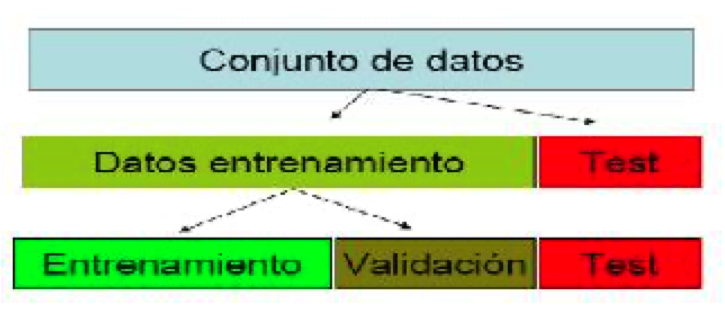
\includegraphics{graficos/DivisionEnt_Val_Test.png}
\caption{División de datos muestrales para entrenamiento, validación y
testeo}
\end{figure}

El conjunto de \emph{datos de entrenamiento} es aquel que utilizamos
para probar diferentes hiperparametrizaciones de cada modelo para ver
cual es la más óptima. La hiperparametrización variará en función de los
parámetros aplicables a cada algoritmo utilizado.

Una vez hayamos entrenado los modelos, pasamos a la fase de validación,
donde aplicaremos a los \emph{datos de validación} los diferentes
algoritmos con la configuración de parámetros que mejor haya funcionado
en el conjunto de datos de entrenamiento.

El modelo con el que obtengamos las mejores métricas será el que
posteriormente apliquemos a los \emph{datos de testeo}, ofreciéndonos el
error real cometido con el modelo seleccionado. Es decir, este último
conjunto de datos se utiliza para estiamr el error de generalización del
modelo, ya que nuestro objetivo es obtener un error de generalización
pequeño evitando el sobreajuste.

A continuación vamos a exponer tres algoritmos de aprendizaje automático
que posteriormente aplicaremos a nuestros datos

\hypertarget{muxe1quinas-de-vector-soporte-support-vector-machines-svms}{%
\subsubsection{Máquinas de vector soporte (Support Vector Machines
SVMs)}\label{muxe1quinas-de-vector-soporte-support-vector-machines-svms}}

Las máquinas de vector soporte son un conjunto de algoritmos de
aprendizaje estadístico supervisado pertenecientes a la familia de los
clasificadores lineales.

Suponiendo que tenemos ejemplos de sólo dos categorías y sin pérdida de
generalidad, una SVM construye un hiperplano en un espacio de
dimensionalidad muy alta. Este hiperplano separa de forma óptima los
puntos de una clase de la otra. La característica fundamental de estos
algoritmos es el concepto de ``separación óptima'', ya que se busca el
hiperplano que tenga la máxima distancia con los puntos que estén más
cerca de él mismo al tiempo que clasifica correctamente tantos puntos de
entrenamiento como sea posible. Los algoritmos SVM representan el
hiperplano óptimo con vectores de soporte.

En nuestro caso al ser la variable volumen de ventas una variable
numérica, vamos a centrarnos en la variante SVM para regresión, tambien
conocida como SVR (support vector regressor). El caso del problema de
regresión es una generalización del problema de clasificación, en la que
el modelo devuelve un valor continuo, es decir, un modelo de regresión
estima una función multivariante de valor continuo.

\hypertarget{descripciuxf3n-del-algoritmo}{%
\paragraph{Descripción del
algoritmo}\label{descripciuxf3n-del-algoritmo}}

Dado un conjunto de ejemplos de entrenamiento
\(S = \big\{(x_1,y_1), \dots,(x_n,y_n)\big\}\), donde
\(x_i \in \mathbb R^d \text{ e }\ y_i \in \mathbb R\), en el que se
asume que todos los valores \(y_i\) de todos los ejemplos de \(S\)
pueden ser ajustados mediante un hiperplano, nuestro objetivo será
encontrar los parámetros \(w = (w_1,\dots,w_d)\) que permitan definir el
hiperplano de regresión
\[y=f(x) = (w_1x_1+\dots+w_dx_d) + b = \langle w,x \rangle+b \text{ , } b \in \mathbb R\]

La generalización de SVM a SVR se logra introduciendo una región
insensible a \(\epsilon\) alrededor de la función. Esta región se conoce
como tubo épsilon. Este tubo reformula el problema de optimización para
encontrar el tubo que mejor se aproxime a la función al tiempo que
equilibra el error de predicción, es decir, se formula un problema de
optimización definiendo una función de pérdida a minimizar insensible a
\(\epsilon\) y encontrando el tubo más plano que contiene a la mayoría
de instancias de entrenamiento.

Se dice \textbf{rudio, perturbación aleatoria o tubo épsilon} y se
representa por \(\epsilon \sim N(0,\sigma^2)\), al error en la medición
del valor \(y\), por tanto, \(y=f(x) + \epsilon\)

El valor de \(\epsilon\) determina el ancho del tubo, y un valor más
pequeño indica menor tolerancia al error, cuando más pequeño sea el
valor de \(\epsilon\), el límite del tubo se desplaza hacia dentro,
habiendo más puntos de datos alrededor del límite, lo que indica más
vectores de soporte.

Se define la \textbf{función de pérdida lineal} \(\epsilon-\)
insensible, y se representa como \(L_{\epsilon}\) a una función lineal
en el que la función de pérdida toma valor nulo y viene definida de la
siguiente forma: \[L_{\epsilon} = 
\begin{cases} 
0 & \text{ si} |y-f(x)| \leq \epsilon, \\ 
|y-f(x)| - \epsilon & \text{ en caso contrario }
\end{cases}\]

\begin{figure}[H]

{\centering 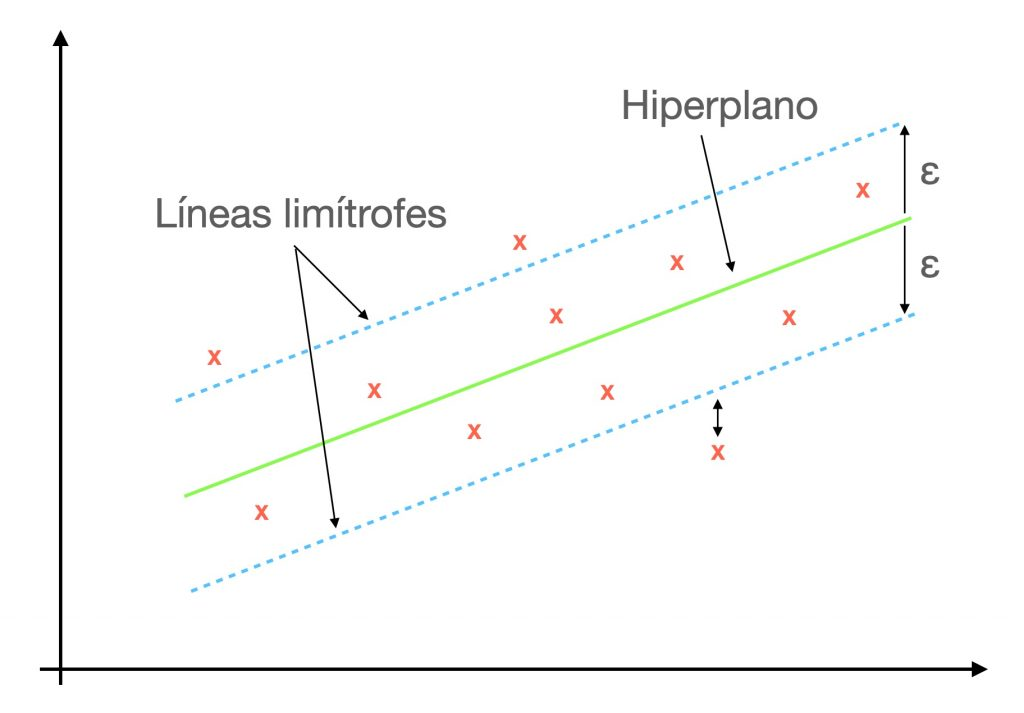
\includegraphics[width=0.95\linewidth]{graficos/svr.jpg } 

}

\caption{Vectores de Soporte de Regresión.}\label{fig:SVR_lu}
\end{figure}

\hypertarget{k-nearest-neighbor-regression-knn}{%
\subsubsection{K-Nearest Neighbor Regression
(KNN)}\label{k-nearest-neighbor-regression-knn}}

El algoritmo de K-vecinos más cercanos, más conocido como KNN, fué
desarrollado en el año 1951 por los matemáticos Evelyn Fix y Andrew
Hodges.

El algoritmo KNN es un método de aprendizaje supervisado que está basado
en criterios de vecindad, por lo que es necesario establecer cierta
medida de distancia entre los diferentes elementos de la representación.
La ventaja de la aplicación de técnicas basadas en la vecindad es la
siguiente: el valor de salida que se otorgará a una nueva instancia se
calculará en función de los valores de los puntos más cercanos a ella.
Se trata de un método local, que asume que la salida de un nuevo dato
depende exclusivamente de los k vecinos de entrenamiento más próximos.

\hypertarget{descripciuxf3n-del-algoritmo-1}{%
\paragraph{Descripción del
algoritmo}\label{descripciuxf3n-del-algoritmo-1}}

Este algoritmo puede ser utilizado para modelos de clasificación y de
regresión, ocupándonos en este trabajo la segunda opción. En el caso de
la clasificación, En se determinará la clase a la que pertenecerá la
nueva instancia en función de la clase mayoritaria de los vecinos más
cercanos del conjunto de entrenamiento; y en regresión, el modelo debe
determinar el valor del nuevo dato como el valor medio de los k ejemplos
de entrenamiento más cercanos, siguiendo la siguiente ecuación del valor
de la nueva instancia de entrada:

\[
Valor(Inst_{\text{entrada}}) = \dfrac{1}{K} \sum_{i=1}^k Valor(P_i)
\]

Como ya habíamos avanzado antes, para determinar cómo de cercanos se
encuentran unas instancias de otras, es necesario definir una medida de
similitud o distancia para todos los datos del conjunto muestral.
Definiremos esta medida de similitud a través de una función, como puede
ser la distancia Manhattan, la distancia Minkow o las más utilizada la
distancia Euclídea, que es la que se va a utilizar, y viene dada por:

\[
d(p,1) = \sqrt{ \sum_{i=1}^n (p_i-q_i)^2}
\]

Una vez definida esta medida, procedemos a la descripción del algoritmo:

\begin{itemize}
\item
  Se almacena el conjunto de datos de entrenamiento compuesto por un
  vector de entrada y otro de salida
\item
  Se establece el valor del parámetro k
\item
  Se presenta una nueva instancia j teniendo en cuenta únicamente el
  vector de entrada de esta nueva instancia

  \begin{itemize}
  \tightlist
  \item
    Se calcula la distancia euclídea de la nueva instancia con todos lso
    datos del conjunto de entrenamiento
  \item
    Se calcula la salida del este nuevo dato como la media de las
    salidas de los k datos más cercanos a él
  \end{itemize}
\item
  Se repite el paso anterior para todas las instancias del conjunto de
  datos
\end{itemize}

\begin{figure}[H]

{\centering 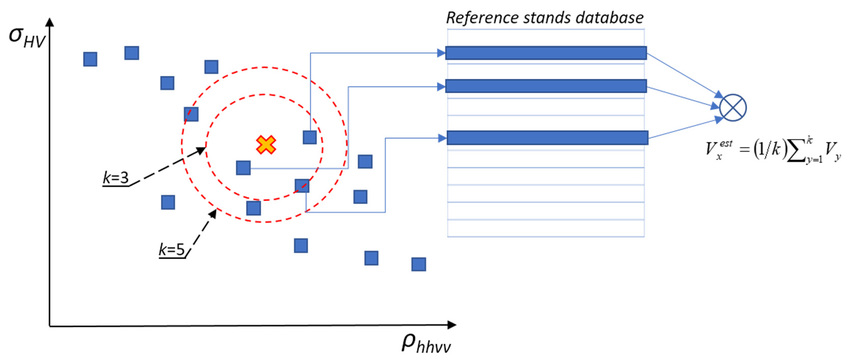
\includegraphics[width=0.95\linewidth]{graficos/knn_regression} 

}

\caption{Esquema conceptual del algoritmo KNN de regresión.}\label{fig:knn_esq}
\end{figure}

En la figura \protect\hyperlink{knn_esq}{4.3} podemos ver un esquema
conceptual del algoritmo, donde el valor de salida que el modelo le dará
al nuevo punto marcado con una \emph{x} será la media de los valores de
los puntos vecinos. Habiéndose seleccionado a modo de ejemplo el valor
de k=3 y k=5.

@ref(fig:bookdownLogo)

\hypertarget{elecciuxf3n-del-paruxe1metro-k}{%
\paragraph{Elección del parámetro
k}\label{elecciuxf3n-del-paruxe1metro-k}}

Es necesario seleccionar el valor que se le va a dar al parámetro k, es
decir, el número de vecinos con los que se realizará la media para
obtener el valor de salida de la nueva instancia. Si este valor es muy
grande, la idea de vecinos que están lejos podrían influir con la nueva
instancia sin tener relación, pero si este valor es demasiado pequeño,
el algoritmo será muy sensible a valores extremos.

\hypertarget{uxe1rboles-de-regresiuxf3n-xgboost-model}{%
\subsubsection{Árboles de regresión (XGBoost
Model)}\label{uxe1rboles-de-regresiuxf3n-xgboost-model}}

\hypertarget{evaluaciuxf3n-y-presentaciuxf3n-de-resultados-anuxe1lisis-del-error}{%
\subsubsection{Evaluación y presentación de resultados (+análisis del
error)}\label{evaluaciuxf3n-y-presentaciuxf3n-de-resultados-anuxe1lisis-del-error}}

\begin{itemize}
\tightlist
\item
  Predicciones con el mejor modelo
\item
  Final de la historia de una forma ordenada y resumida
\item
  Señalar posibles mejoras y recomendaciones para proyectos futuros
\end{itemize}

\FloatBarrier

\appendix

\ifdefined\ifprincipal
\else
\setlength{\parindent}{1em}
\pagestyle{fancy}
\setcounter{tocdepth}{4}
\tableofcontents

\fi

\ifdefined\ifdoblecara
\fancyhead{}{}
\fancyhead[LE,RO]{\scriptsize\rightmark}
\fancyfoot[LO,RE]{\scriptsize\slshape \leftmark}
\fancyfoot[C]{}
\fancyfoot[LE,RO]{\footnotesize\thepage}
\else
\fancyhead{}{}
\fancyhead[RO]{\scriptsize\rightmark}
\fancyfoot[LO]{\scriptsize\slshape \leftmark}
\fancyfoot[C]{}
\fancyfoot[RO]{\footnotesize\thepage}
\fi
\renewcommand{\headrulewidth}{0.4pt}
\renewcommand{\footrulewidth}{0.4pt}

\hypertarget{apuxe9ndice-tuxedtulo-del-apuxe9ndice}{%
\chapter{Apéndice: Título del
Apéndice}\label{apuxe9ndice-tuxedtulo-del-apuxe9ndice}}

\hypertarget{primera-secciuxf3n}{%
\section{Primera sección}\label{primera-secciuxf3n}}

\ifdefined\ifprincipal
\else
\setlength{\parindent}{1em}
\pagestyle{fancy}
\setcounter{tocdepth}{4}
\tableofcontents

\fi

\ifdefined\ifdoblecara
\fancyhead{}{}
\fancyhead[LE,RO]{\scriptsize\rightmark}
\fancyfoot[LO,RE]{\scriptsize\slshape \leftmark}
\fancyfoot[C]{}
\fancyfoot[LE,RO]{\footnotesize\thepage}
\else
\fancyhead{}{}
\fancyhead[RO]{\scriptsize\rightmark}
\fancyfoot[LO]{\scriptsize\slshape \leftmark}
\fancyfoot[C]{}
\fancyfoot[RO]{\footnotesize\thepage}
\fi
\renewcommand{\headrulewidth}{0.4pt}
\renewcommand{\footrulewidth}{0.4pt}

\hypertarget{apuxe9ndice-tuxedtulo-del-apuxe9ndice-1}{%
\chapter{Apéndice: Título del
Apéndice}\label{apuxe9ndice-tuxedtulo-del-apuxe9ndice-1}}

\hypertarget{primera-secciuxf3n-1}{%
\section{Primera sección}\label{primera-secciuxf3n-1}}

\FloatBarrier
\cleardoublepage

\ifdefined\ifdoblecara
  \fancyhead[LE,RO]{}
  \fancyfoot[LO,RE]{}
  \fancyhead[CO,CE]{Bibliografía}
\else
  \fancyhead[RO]{}
  \fancyfoot[LO]{}
  \fancyhead[CO]{Bibliografía}
\fi

\ifdefined\ifcitapandoc

\hypertarget{bibliografuxeda}{%
\chapter*{Bibliografía}\label{bibliografuxeda}}
\addcontentsline{toc}{chapter}{Bibliografía}

\else

\textbackslash nocite\{ Luque2017,Luque2019,RStudio,R-base,
R-knitr,R-dplyr,R-ggplot2, MestaTFG,CampoTFG, DefSectorRetail,
ST\_Apuntes, ST\_Art, PEREZ-MARTINEZ2021\_CV, IntroFeatureSelection,
EDA, SVM\_CampoTFG, SVM\_SVR, KNN\_R\_TFG \}

\fi

\bibliography{bib/library.bib,bib/paquetes.bib}


\addcontentsline{toc}{chapter}{Bibliografía}


\end{document}
